\chapter{Descrizione della zona in esame e degli eventi studiati}

\section{Sismicità e tettonica della Kamchatka}
La penisola della Kamchatka è una regione della Russia orientale situata nel nord-ovest del Pacifico, lunga \qty{1250}{\kilo\meter} (\(51-61^\circ \text{N}\)) e larga \qty{450}{\kilo\meter} (\(155-163 ^\circ \text{E}\)) \citep{glacier_mass}. Questa zona è tra le più sismicamente attive del pianeta. Infatti, dall'inizio del secolo scorso sono stati registrati diversi grandi terremoti, inclusi sei eventi con magnitudo superiore a 8: nel 1904 (\(M_s = 8.0\)), 1923 (\(M_w = 8.5\)), 1952 (\(M_w = 9.0\)), 1959 (\(M_w = 8.2\)), 1997 (\(M_w = 7.8\)) e nel 2025 (\(M_w = 8.8\)). In particolare il terremoto del 1952 è il quinto terremoto più potente che sia stato registrato fino ad ora.

Questa regione fa parte dell'arco delle Curili-Kamchatka, che si estende per circa \qty{2100}{\kilo\meter}, partendo da Hokkaido in Giappone, passando per le isole Curili e la penisola della Kamchatka, terminando intersecandosi con l'arco delle isole Aleutine, a sud delle isole del Commodoro in Russia. 
L'arco delle Curili-Kamchatka indica la zona in cui la placca del Pacifico subduce nel mantello sotto la placca Nordamericana con un rate di \(77~\mathrm{mm/yr}\) vicino alla parte settentrionale dell'arco (\(55 ^\circ \text{N}\)) fino a \(83~\mathrm{mm/yr}\) nella zona prossima ad Hokkaido (\(47 ^\circ \text{N}\)) \citep{description}.

Studiando la struttura litosferica lungo la costa orientale della Kamchatka è stato stimato che la crosta abbia uno spessore tra i \qty{30}{\kilo\meter} e i \qty{40}{\kilo\meter}, tramite misure di gravità e rilevazioni sismiche a sorgente attiva \citep{bogdanov2000tectonic} e modelli di funzioni di ricevitore teleseismiche \citep{levin2002}. 
Tali spessori sono comparabili alla profondità dei terremoti generati da faglie di sovrascorrimento lungo la placca subdotta, evidenziando il legame tra struttura litosferica e sismicità nella regione. 
L'arco delle Curili-Kamchatka è infatti una delle aree più sismicamente attive al mondo: la deformazione della placca Nordamericana sovrastante genera terremoti crostali poco profondi, mentre lo scorrimento lungo il piano di subduzione tra la placca Pacifica e quella Nordamericana produce terremoti che si estendono fino a profondità di 40–60 km \citep{usgs2025qw60}.

La morfologia della placca del Pacifico cambia a \(53.5-54.5 ^\circ \text{N}\), quando questa incontra il monte sottomarino Meiji (Meiji Seamount), cambiando il carattere della subduzione. L'angolo di subduzione decresce da sud a nord da \(55 ^\circ\) a \(35 ^\circ\) e la massima profondità della sismicità si riduce da \(\sim\) \qty{600}{\kilo\meter} a \(\sim\) \qty{200}{\kilo\meter}, provocando una deviazione verso nord-ovest del fronte vulcanico \citep{description, usgs2025qw60}.

\section{Attività vulcanica in Kamchatka}
I vulcani sulla superficie terrestre non sono distribuiti casualmente. La maggior parte di questi si trova ai margini dei continenti, lungo catene di isole, o sotto il livello del mare dove formano lunghe catene montuose. In particolare, più della metà dei vulcani attivi si trova nell'oceano Pacifico \citep{usgs_volcanoes_plate_tectonics_1997} e forma quella che viene chiamata ''Cintura di Fuoco'', che circonda il Pacifico passando proprio per la Kamchatka.
Si nota infatti, una certa correlazione tra i confini delle placche tettoniche e la formazione di catene vulcaniche, come mostrato in Fig.\ref{fig:fire_ring} \citep{encyclopedia}.
La penisola della Kamchatka è proprio tra le regioni con la più alta attività vulcanica del pianeta; attiva da più di \qty{70}{Ma} a causa della subduzione della placca oceanica del Pacifico sotto la placca continentale Nordamericana \citep{volcan_kam}.

\begin{figure}[H]
    \centering
    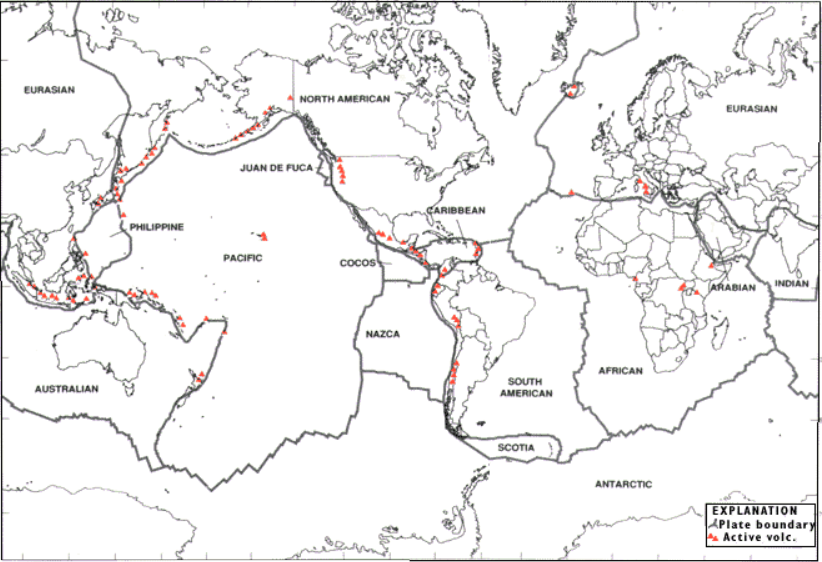
\includegraphics[width=0.75\linewidth]{graphics/fire_ring.png}
    \caption{Mappa indicante i confini delle placche e la posizione di diversi vulcani in attività [preso da U. S. Geological Survey (\citeyear{usgs_volcanoes_plate_tectonics_1997})]}
    \label{fig:fire_ring}
\end{figure}

La teoria della tettonica a placche riesce a spiegare i meccanismi principali della produzione di magma e quindi l'attività vulcanica che ne consegue.
La formazione del magma avviene principalmente in due modi: il primo consiste nella decompressione di materiale solido e caldo dal mantello, il secondo si basa invece sull'aggiunta di componenti volatili, tra cui principalmente H\(_2\)O, per abbassare la temperatura di fusione del mantello.
La decompressione del magma, in particolare, viene prodotta dai pennacchi (mantle plumes) e dai margini convergenti.
I pennacchi sono colonne ascendenti di materiale roccioso proveniente dalla parte bassa del mantello. Risalendo, tipicamente a basse profondità (\(<\)\qty{200}{\kilo\meter}) \citep{encyclopedia}, incontrano le giuste condizioni di pressione e temperatura che portano alla fusione del materiale solido e alla formazione di magma.
Per quanto riguarda i margini divergenti, il mantello, compiendo dei moti convettivi, risale lentamente (\(\mathrm{cm/yr}\)) fino a \(\sim\) \qty{60}{\kilo\meter} dalla superficie, dove inizia a fondere a causa di una diminuzione della pressione \citep{earle_plate_tectonics_2021}. Poiché si tratta di margini divergenti, il magma prodotto va a riempire lo spazio creato dalla rimozione laterale della litosfera, contribuendo alla formazione di nuova crosta oceanica.
Lungo i margini convergenti la formazione del magma avviene a seguito della subduzione della litosfera oceanica nel mantello. La litosfera oceanica, nonostante sia più fredda del mantello, è anche ricca di acqua; durante la subduzione, i fluidi vengono rilasciati nel mantello sovrastante, abbassandone il punto di fusione e favorendo la generazione di un magma generalmente ricco di gas.
L'arco delle Curili-Kamchatka è un esempio di attività vulcanica generata dalla subduzione della litosfera oceanica della placca del Pacifico sotto la litosfera oceanica della placca Nordamericana. Quando due croste oceaniche convergono, una delle due viene subdotta sotto l'altra e il  magma prodotto dalla crosta subdotta nel mantello risale attraverso la crosta oceanica sovrastante, formando un arco di isole vulcaniche.

Nello specifico la penisola della Kamchatka è costituita da tre fronti vulcanici:: lo Sredinny Range, l’Eastern Volcanic Front (EVF) e la Central Kamchatka Depression (CKD).

...


\section{Terremoto M8.8 del 29/07/2025}
Il 29 luglio 2025 (30 luglio alle 11:24 ora locale) si è verificato un terremoto \(M_w = 8.8\), tra i 10 più potenti mai registrati, prodotto dalla stessa zona di subduzione che generò nel 1952 un terremoto \(M_w = 9.0\).
Terremoti di questa magnitudo si verificano in prossimità di zone di subduzione e sono generati da una faglia detta di \textit{mega sovrascorrimento} (\textit{megathrust}). Questa separa due placche convergenti, quella del Pacifico che subduce a quella nordamericana \citep{jk0}.

Terremoti di questa portata sono eventi piuttosto rari. In un loro articolo, \citet{jk1} prendono in considerazione i diciassette terremoti di magnitudo \(M_w=8.5\) e maggiori avvenuti dal 1900 ad oggi. La loro analisi prosegue cercando una dipendenza tra questi eventi e i \textit{foreshock}, terremoti di minore entità che ne precedono uno maggiore, in particolare ricercando la correlazione tra foreshock di magnitudo \(M_w=7+\) e gli eventi di magnitudo  \(M_w=8.5+\).
Ne risulta però che la correlazione è di \(\sim1 \%\), mostrando che questi eventi sono difficili da prevedere attraverso l'analisi dei foreshock.




\begin{figure}[H]
    \centering
    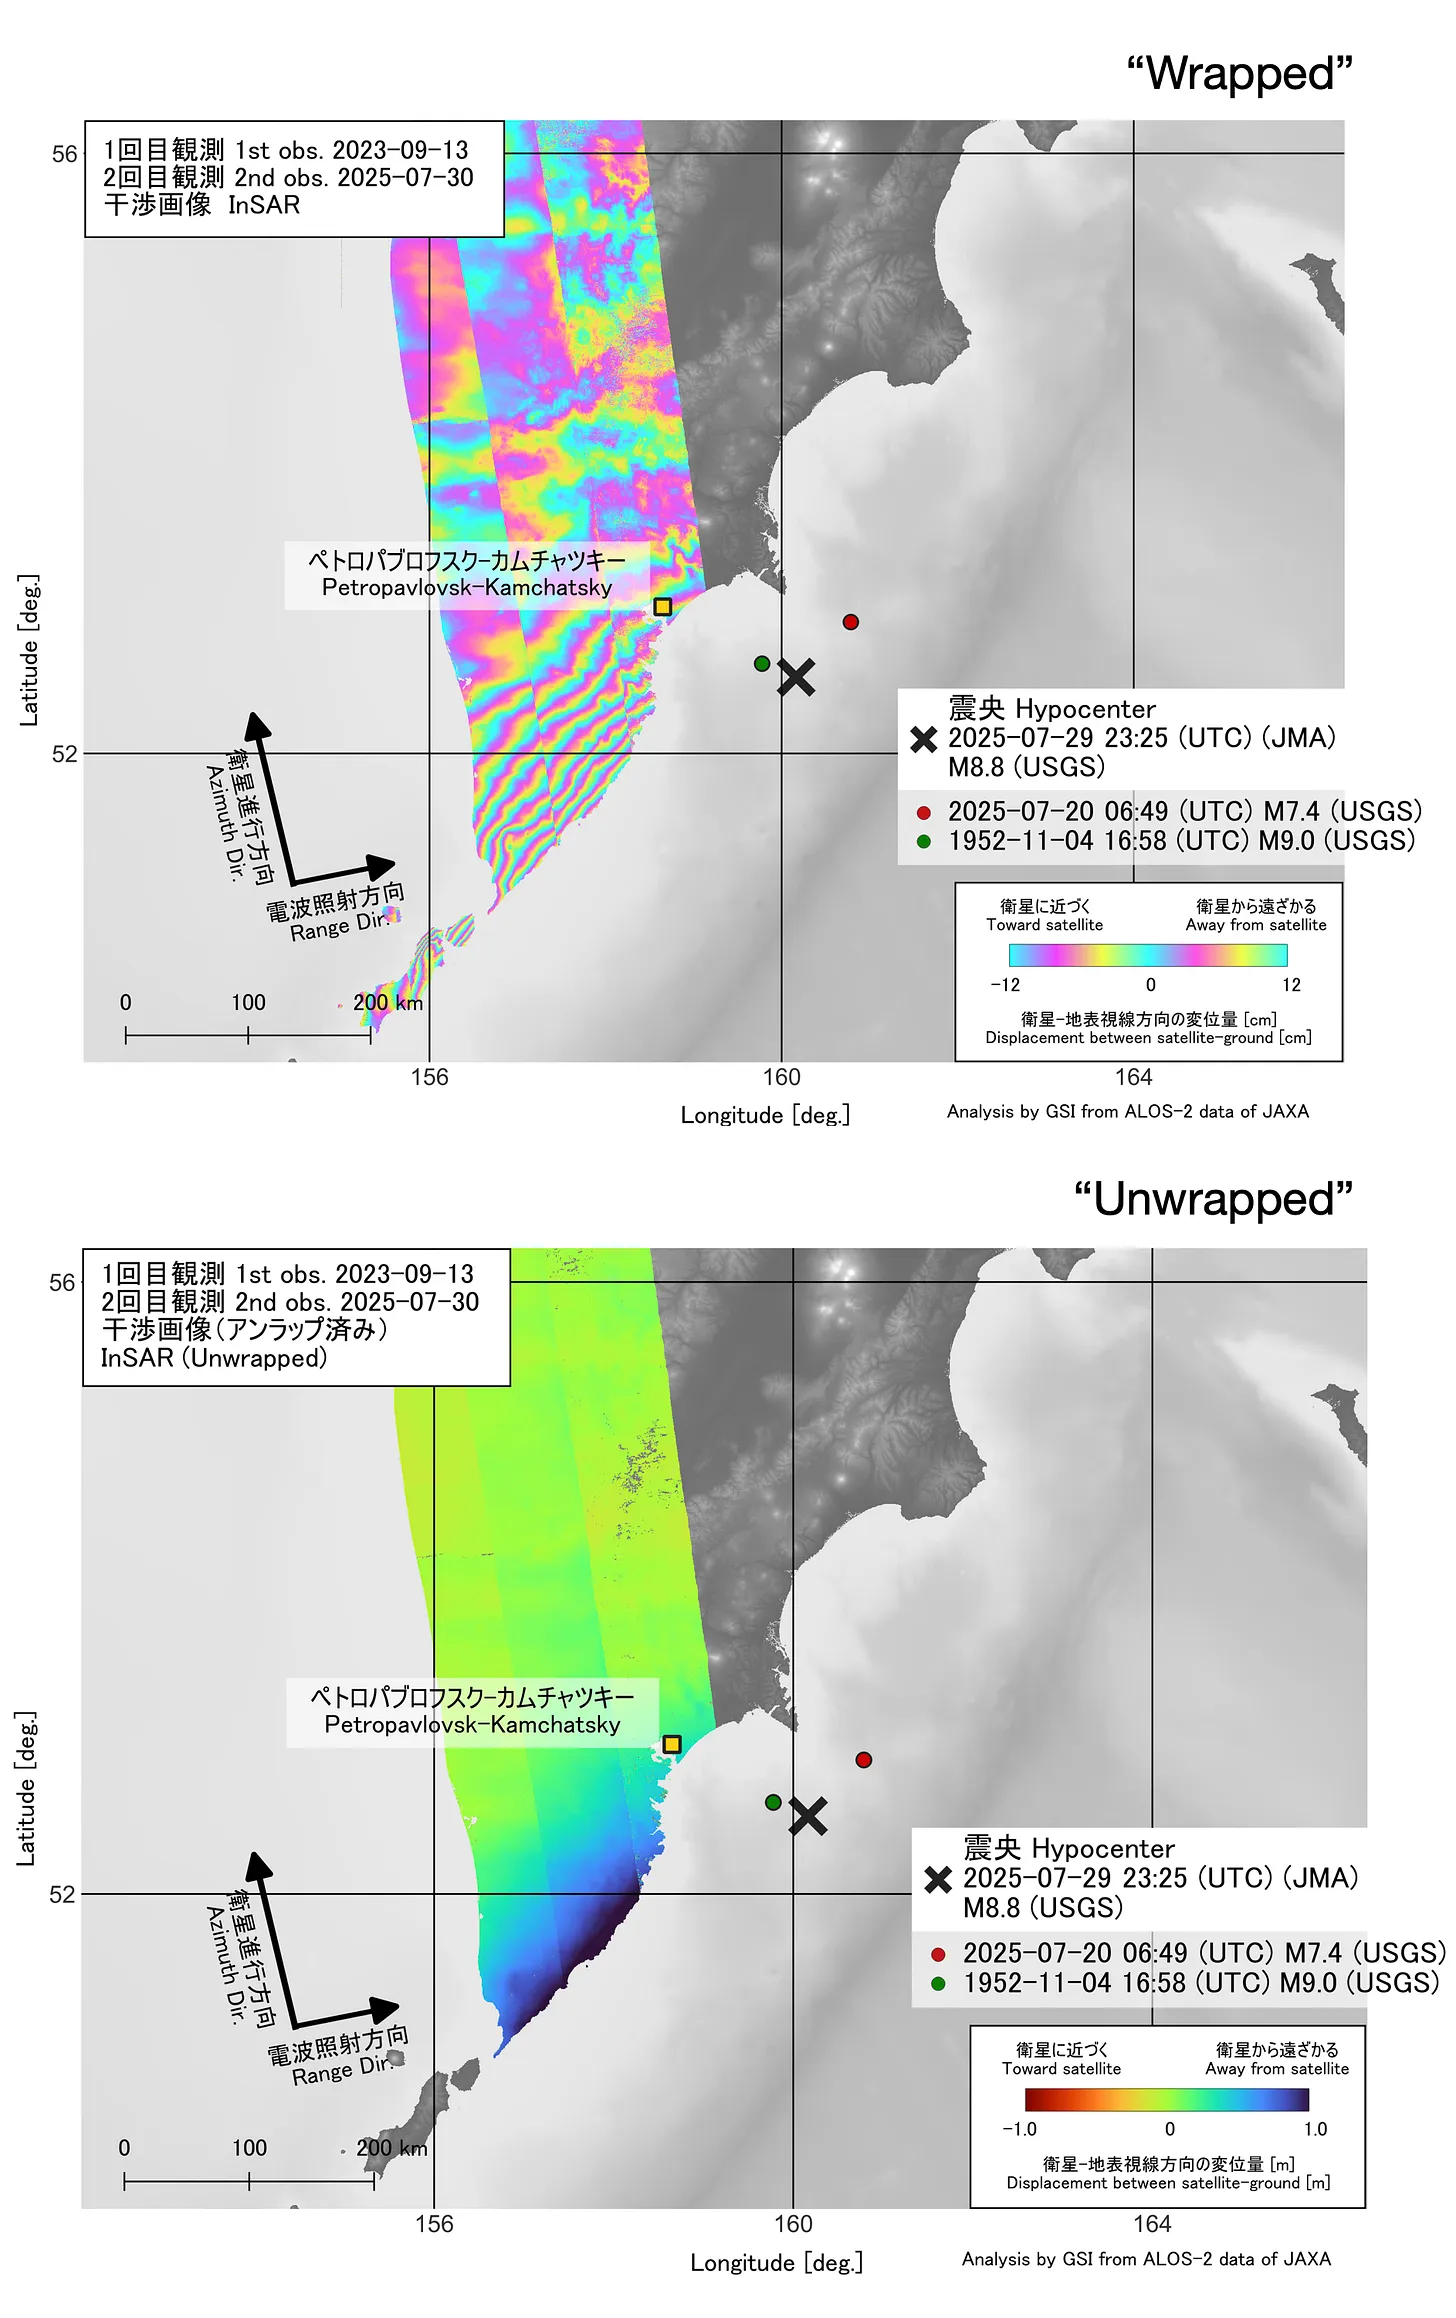
\includegraphics[width=0.7\linewidth]{graphics/wrap_unwrap.png}
    \caption{Caption}
    \label{fig:placeholder}
\end{figure}

\begin{figure}[H]
    \centering
    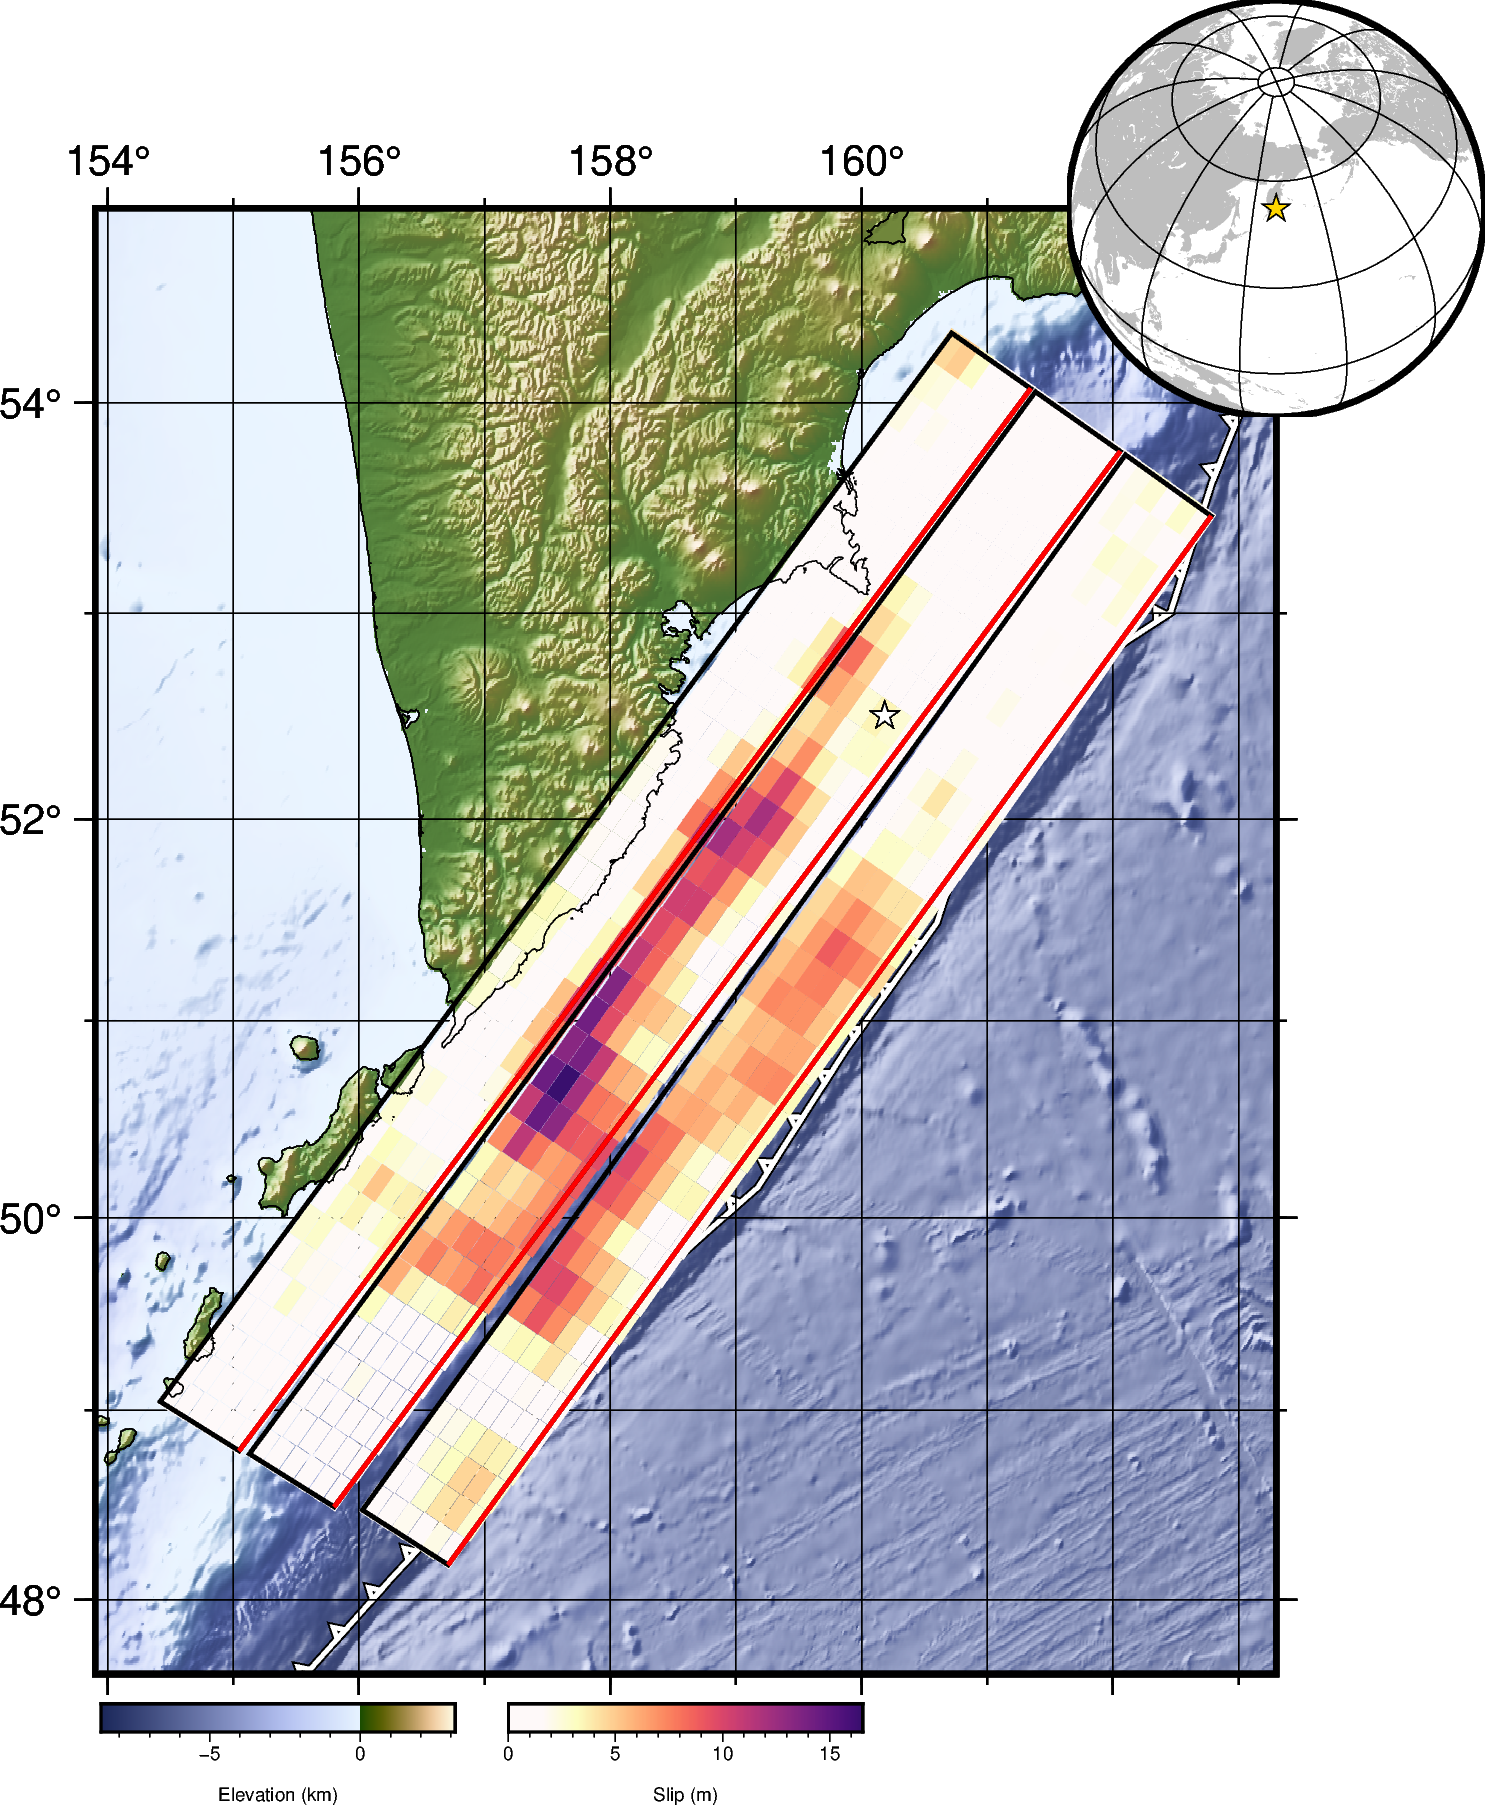
\includegraphics[width=0.7\linewidth]{graphics/00.png}
    \caption{Caption}
    \label{fig:00}
\end{figure}

\begin{figure}[H]
    \centering
    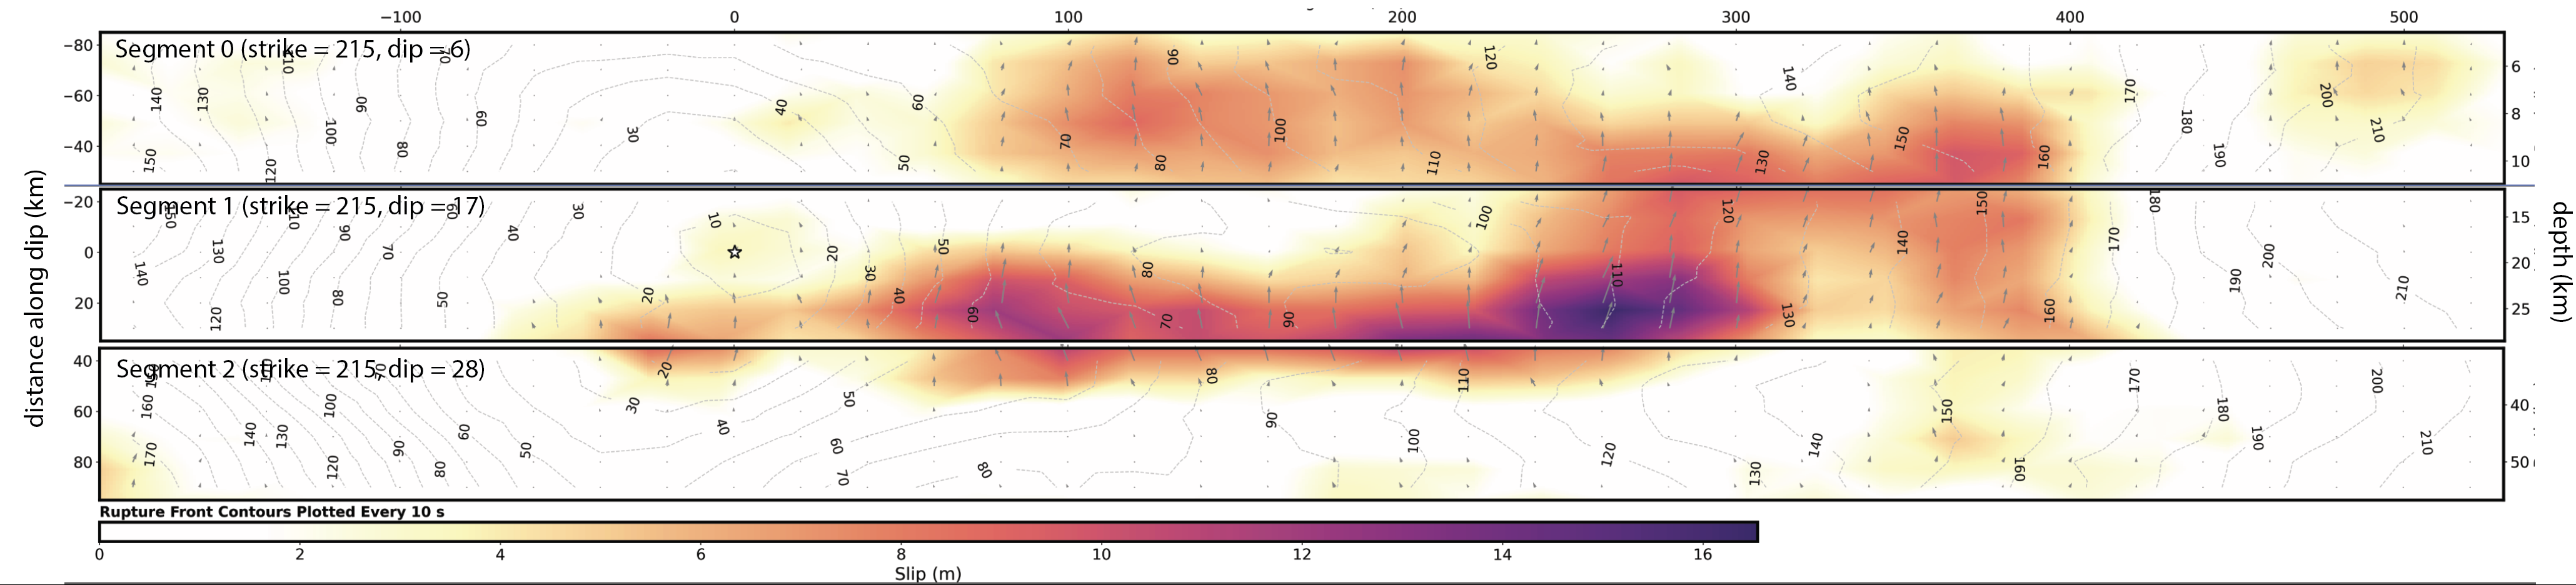
\includegraphics[width=0.7\linewidth]{graphics/01.png}
    \caption{Caption}
    \label{fig:01}
\end{figure}

\begin{figure}[H]
    \centering
    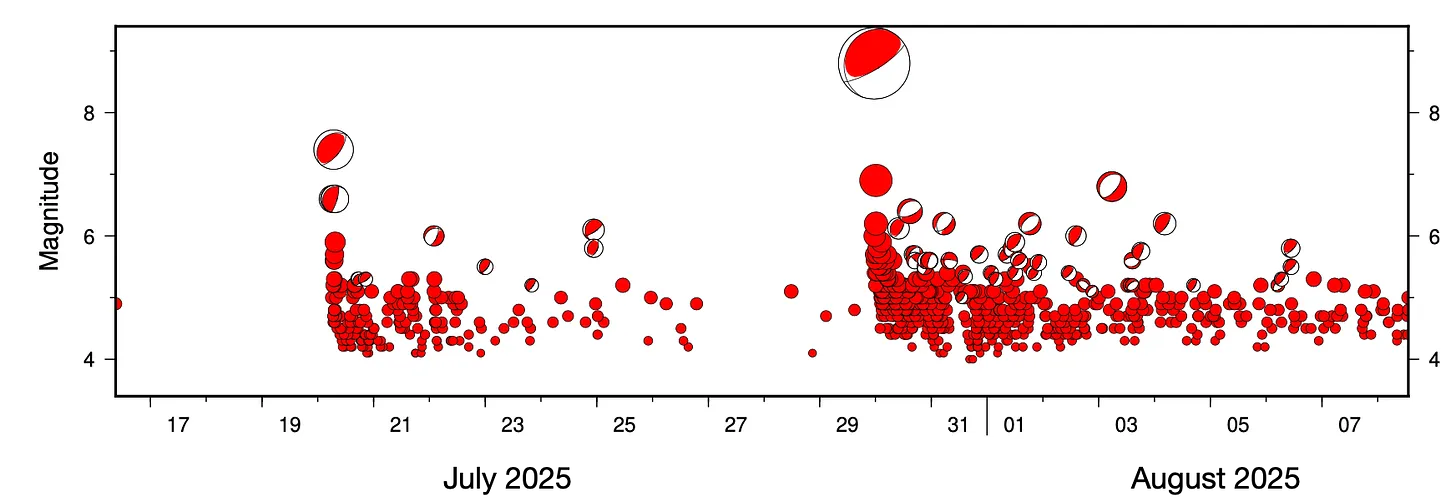
\includegraphics[width=0.7\linewidth]{graphics/111.png}
    \caption{Caption}
    \label{fig:1}
\end{figure}

\begin{figure}[H]
    \centering
    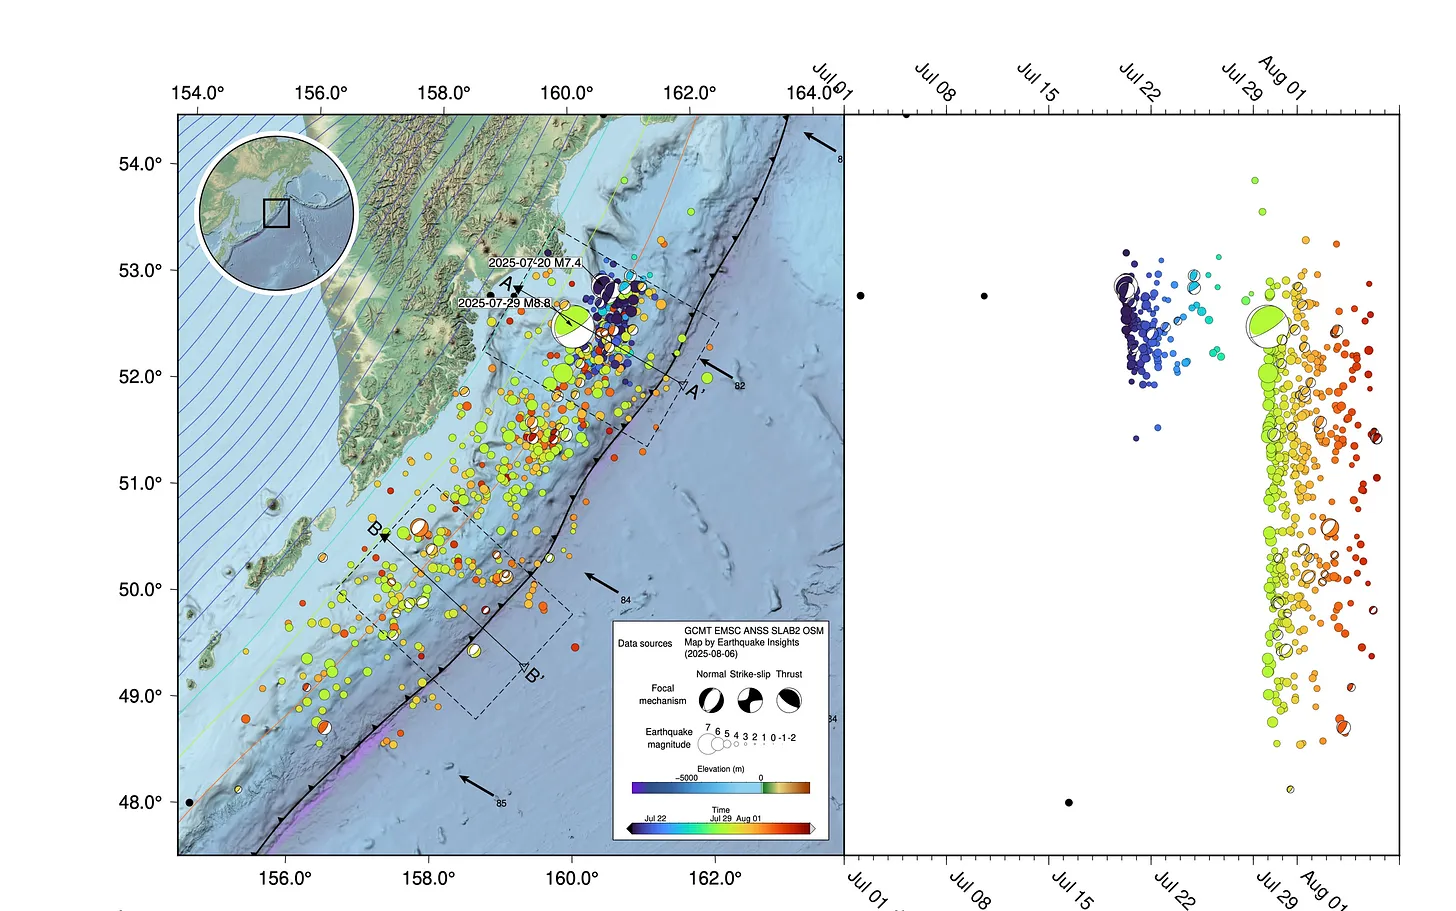
\includegraphics[width=0.7\linewidth]{graphics/222.png}
    \caption{Caption}
    \label{fig:2}
\end{figure}

\begin{figure}[H]
    \centering
    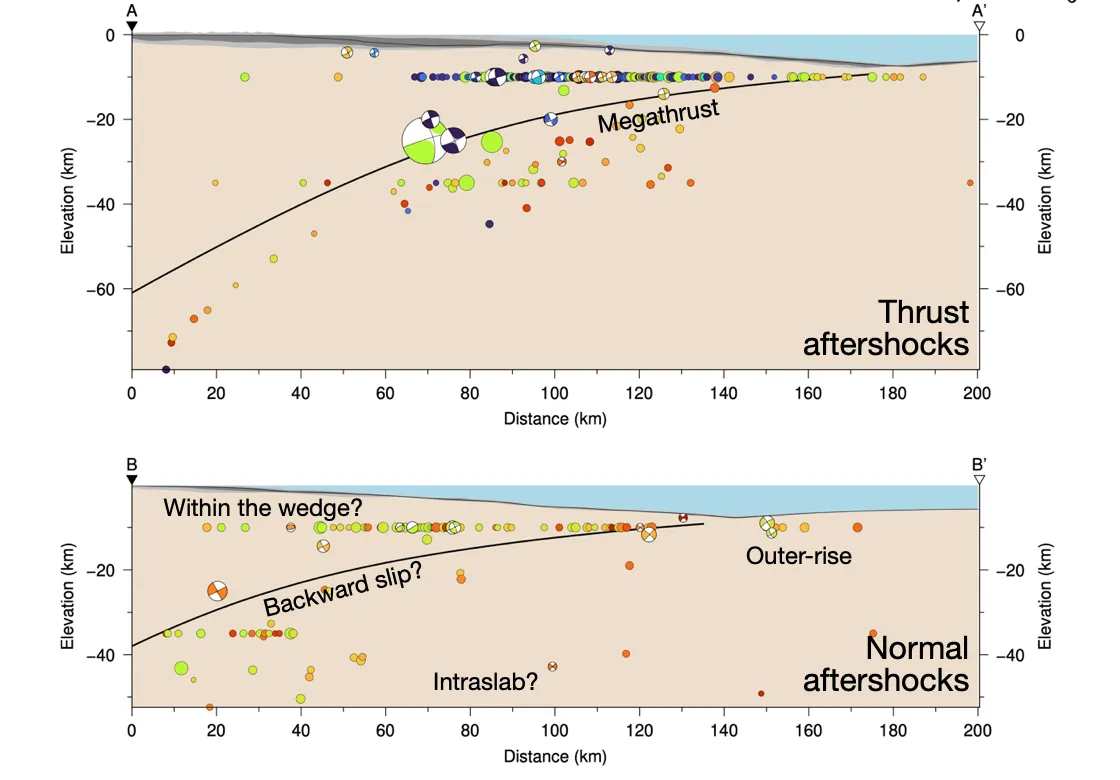
\includegraphics[width=0.7\linewidth]{graphics/333.png}
    \caption{Caption}
    \label{fig:3}
\end{figure}

\begin{figure}[H]
    \centering
    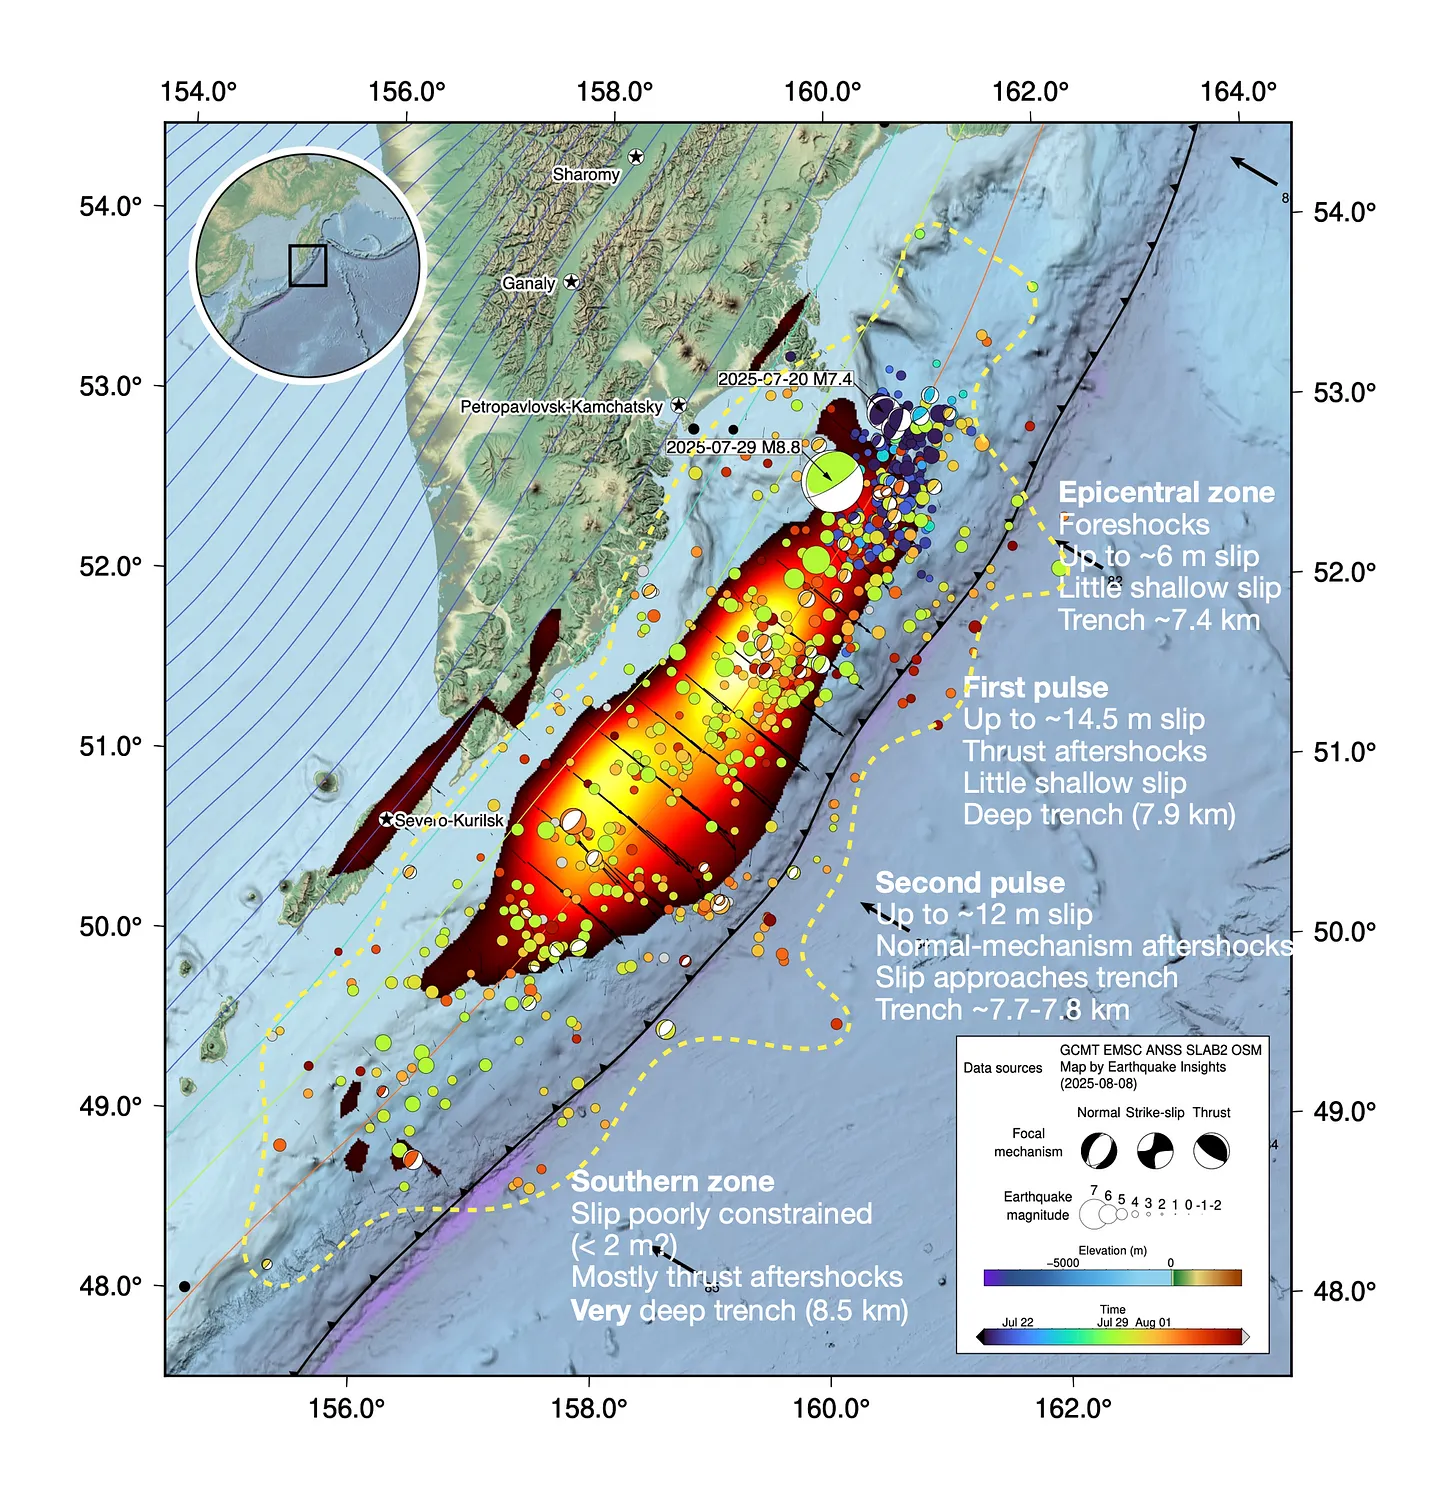
\includegraphics[width=0.7\linewidth]{graphics/444.png}
    \caption{Caption}
    \label{fig:4}
\end{figure}



\section{Vulcani}

\subsection{Vulcano 1}

\subsection{Vulcano 2}

